\documentclass[11pt]{article}
% BEGIN SHARED COURSE STYLE
% Shared Math 615 style. Embedded verbatim in standalone published sources.
\RequirePackage[letterpaper,margin=1in]{geometry}
\RequirePackage{amsmath,amsthm,mathtools}
\RequirePackage{fontspec,unicode-math}
\setmainfont{texgyretermes}[Extension=.otf,UprightFont=*-regular,BoldFont=*-bold,ItalicFont=*-italic,BoldItalicFont=*-bolditalic]
\setmathfont{texgyretermes-math.otf}
\RequirePackage{microtype,tikz-cd,enumitem,needspace,xcolor,booktabs,titlesec,etoolbox}
\definecolor{teal}{HTML}{176568}
\definecolor{burgundy}{HTML}{782F40}
\definecolor{inklink}{HTML}{176568}
\definecolor{accent}{HTML}{176568}
\titleformat{\section}{\large\bfseries\color{teal}}{\thesection}{.65em}{}
\titleformat{\subsection}{\normalsize\bfseries\color{burgundy}}{\thesubsection}{.65em}{}
\titleformat{\paragraph}[runin]{\normalsize\bfseries\color{burgundy}}{}{0pt}{}
\titlespacing*{\section}{0pt}{4ex plus 1ex minus .5ex}{1.5ex plus .3ex}
\titlespacing*{\subsection}{0pt}{3ex plus .8ex minus .4ex}{1ex plus .2ex}
\RequirePackage{hyperref,bookmark}
\hypersetup{colorlinks=true,linkcolor=teal,urlcolor=teal,citecolor=teal,pdfstartview={XYZ null null 1.5},bookmarksnumbered=true}
\urlstyle{same}
\setcounter{tocdepth}{2}
\setlist[enumerate]{label=\arabic*.,ref=\arabic*,leftmargin=*,itemsep=4pt,topsep=4pt}
\setlength{\parindent}{1em}
\setlength{\parskip}{3pt}
\setlength{\emergencystretch}{2em}
\raggedbottom
\AddToHook{cmd/section/before}{\Needspace{8\baselineskip}}
\AddToHook{cmd/subsection/before}{\Needspace{6\baselineskip}}
\makeatletter
\newcommand{\afterblock}{\@afterindentfalse\@afterheading}
\makeatother
\newcounter{result}[section]
\renewcommand{\theresult}{\thesection.\arabic{result}}
\newcommand{\resulttitle}[3]{#1 #2\ifstrempty{#3}{}{ (#3)}.}
\newenvironment{result}[3]{\par\addvspace{7pt}\Needspace{4\baselineskip}\refstepcounter{result}\hypertarget{#2}{}\label{#2}\noindent{\color{burgundy}\hypersetup{linkcolor=burgundy}\hyperlink{proof:#2}{\textbf{\resulttitle{#1}{\theresult}{#3}}}}\quad\ignorespaces}{\par\addvspace{4pt}\afterblock}
\newenvironment{entry}[3]{\par\addvspace{7pt}\Needspace{3\baselineskip}\refstepcounter{result}\hypertarget{#2}{}\label{#2}\noindent{\color{burgundy}\textbf{\resulttitle{#1}{\theresult}{#3}}}\quad\ignorespaces}{\par\addvspace{4pt}\afterblock}
\newenvironment{demonstration}[1]{\par\noindent\hypertarget{proof:#1}{}{\color{burgundy}\hypersetup{linkcolor=burgundy}\hyperlink{#1}{\textbf{Proof.}}}\quad\ignorespaces}{\unskip\nobreak\hfill\qedsymbol\par\addvspace{5pt}\afterblock}
\newenvironment{citedresult}[4]{\par\addvspace{7pt}\Needspace{4\baselineskip}\refstepcounter{result}\hypertarget{#2}{}\label{#2}\noindent{\color{burgundy}\hypersetup{urlcolor=burgundy}\href{#4}{\textbf{\resulttitle{#1}{\theresult}{#3}}}}\quad\ignorespaces}{\par\addvspace{4pt}\afterblock}
\newcommand{\usedby}[1]{\par\noindent{\small\textbf{Used in:} #1.}\par\afterblock}
\newcommand{\coursebold}[1]{{\color{burgundy}\textbf{#1}}}
\newcommand{\coursetitle}[3]{\begin{center}{\large\bfseries\color{teal}#1}\\[4pt]{\LARGE\bfseries\color{teal}#2}\\[6pt]Math 615: Algebraic Topology I\\Fall 2026\quad\textbar\quad #3\end{center}}
\newcommand{\coursecontents}{{\small\setlength{\parskip}{0pt}\tableofcontents}}
\newcommand{\homeworkstyle}{\titleformat{\section}{\large\bfseries\color{teal}}{Exercise \thesection.}{.65em}{}}
% END SHARED COURSE STYLE
\newcommand{\Z}{\mathbb Z}
\newcommand{\mapdef}[5]{#1:#2\longrightarrow #3,\qquad #4\longmapsto #5}
\newcommand{\Top}{\mathrm{Top}}
\newcommand{\Ab}{\mathrm{Ab}}
\hypersetup{pdftitle={Lecture 6: Homotopy Invariance and First Computations},pdfauthor={Math 615 Fall 2026},pdfsubject={Revision 23}}
\begin{document}
\coursetitle{Lecture 6}{Homotopy Invariance and First Computations}{October 5 and 7}
The preceding lecture introduced generalized homology and its axioms. We now verify homotopy invariance and additivity for ordinary singular homology. A homotopy sweeps a singular simplex through a prism. To obtain a chain homotopy, we cut that prism into simplices and take their signed sum. The top and bottom give the two endpoint maps; the faces inside the prism cancel; the vertical sides give the prisms on the boundary. This is the geometric content of homotopy invariance.

We work with integer coefficients and put chain groups in negative degrees equal to zero. Write $I=[0,1]$. All simplex vertices are standard basis vectors. The index conventions used throughout the prism proof are:
\[
\begin{array}{c l}
 n&\text{dimension of the base simplex},\\
 i&\text{a base vertex or a base face},\\
 j&\text{a prism simplex, with the base vertex }e_j\text{ repeated},\\
 k&\text{a vertex position in that prism simplex}.
\end{array}
\]
Barycentric coordinates are $t_0,t_1,\ldots$; the interval coordinate is $t$. A superscript on $d^i$ specifies the omitted vertex. The source and target specify its dimension. The same convention applies to $\tau_j$.
\coursecontents

\section{Singular Homology and the Prism Proof}\label{sec:singular-homology}
\subsection{Singular Chains and Homotopy Invariance}
The standard simplex is the following subspace of $\mathbb R^{n+1}$:
\[
\lvert\Delta^n\rvert=\left\{(t_0,\ldots,t_n):t_i\ge0,\ \sum_{i=0}^nt_i=1\right\}.
\]
Its vertices are $e_0,\ldots,e_n$, and a point has the unique expression $x=\sum_{i=0}^nt_ie_i$. The numbers $t_i$ are its barycentric coordinates. A singular $n$-simplex of $X$ is a continuous map
\[
\sigma:\lvert\Delta^n\rvert\longrightarrow X.
\]
The group $C_n(X)$ is free abelian on these maps. We also write $\sigma$ for its generator in $C_n(X)$.

For $n\ge1$ and $0\le i\le n$, define the affine face inclusion by
\[
\mapdef{d^i}{\lvert\Delta^{n-1}\rvert}{\lvert\Delta^n\rvert}
{(t_0,\ldots,t_{n-1})}{(t_0,\ldots,t_{i-1},0,t_i,\ldots,t_{n-1})}.
\]
The differential is the homomorphism specified on generators by
\[
\mapdef{\partial_n}{C_n(X)}{C_{n-1}(X)}
{\sigma}{\sum_{i=0}^n(-1)^i\sigma d^i}\qquad(n\ge1),
\]
The degree-zero differential is the zero homomorphism
\[
\partial_0:C_0(X)\longrightarrow0.
\] The face identities give $\partial_{n-1}\partial_n=0$. Define
\[
H_n(X)=\ker(\partial_n)/\operatorname{im}(\partial_{n+1}).
\]
A continuous map and its induced maps are
\[
f:X\longrightarrow Y,
\qquad \mapdef{f_{\#,n}}{C_n(X)}{C_n(Y)}{\sigma}{f\sigma},
\]
\[
\mapdef{f_{*,n}}{H_n(X)}{H_n(Y)}{[z]}{[f_{\#,n}(z)]}.
\]
Postcomposition commutes with faces, so $f_\#$ is a chain map. We omit degree subscripts when the source and target specify them.

\label{sec:result}
\begin{result}{Theorem}{thm:prism}{Homotopy Invariance}
Suppose that
\[
f_0,f_1:X\longrightarrow Y,\qquad h:X\times I\longrightarrow Y
\]
satisfy $h(x,0)=f_0(x)$ and $h(x,1)=f_1(x)$. There are homomorphisms
\[
P_n:C_n(X)\longrightarrow C_{n+1}(Y)\qquad(n\ge0)
\]
with $P_{-1}=0$ and
\begin{equation}\label{eq:prism}
\partial_{n+1}P_n+P_{n-1}\partial_n
=f_{1,\#,n}-f_{0,\#,n}:C_n(X)\longrightarrow C_n(Y).
\end{equation}
Thus singular homology is a homotopy invariant functor in each degree:
\[
H_n:\Top\longrightarrow\Ab.
\]
\end{result}
\begin{demonstration}{thm:prism}
The prism operator is constructed in Definition~\ref{def:prism-operator}; Proposition~\ref{prop:boundary-identity} proves \eqref{eq:prism}. For a cycle $z$, that identity gives
\[
f_{1,\#,n}(z)-f_{0,\#,n}(z)=\partial_{n+1}P_n(z).
\]
The two images therefore represent the same homology class. The geometric construction and its boundary calculation follow.
\end{demonstration}

\subsection{Cutting the Prism Into Simplices}\label{sec:details}
Fix $n\ge0$. For each $j=0,\ldots,n$, the $j$th prism simplex has the ordered vertices
\[
(e_0,0),\ldots,(e_j,0),(e_j,1),\ldots,(e_n,1).
\]
Write $s_i=(e_i,0)$ for the bottom vertices. The affine parametrization is
\[
\tau_j:\lvert\Delta^{n+1}\rvert\longrightarrow\lvert\Delta^n\rvert\times I,
\qquad
\tau_j(e_k)=
\begin{cases}
(e_k,0),&0\le k\le j,\\
(e_{k-1},1),&j+1\le k\le n+1.
\end{cases}
\]
The $e_k$ on the left is a standard vertex of the source; those on the right are standard vertices of the base. Affine extension gives the coordinate formula
\[
\tau_j:\lvert\Delta^{n+1}\rvert\longrightarrow\lvert\Delta^n\rvert\times I,
\]
\[
\tau_j(t_0,\ldots,t_{n+1})
=\left(\sum_{k=0}^jt_ke_k+\sum_{k=j+1}^{n+1}t_ke_{k-1},\ \sum_{k=j+1}^{n+1}t_k\right).
\]
Thus $\tau_j$ identifies the two source coordinates in positions $j,j+1$ in the base, and adds the coordinates after position $j$ to obtain the height.

\begin{entry}{Remark}{rem:prism-pieces}{Prism Pieces}
For a point $(x,t)$ in the prism, now write $x=\sum_{i=0}^nt_ie_i$. It belongs to the $j$th piece exactly when
\begin{equation}\label{eq:piece}
\sum_{i=j+1}^nt_i\ \le t\ \le\sum_{i=j}^nt_i.
\end{equation}
Indeed, the unique coordinates in the source of $\tau_j$ are
\[
\left(t_0,\ldots,t_{j-1},\
\sum_{i=j}^nt_i-t,\
 t-\sum_{i=j+1}^nt_i,\
 t_{j+1},\ldots,t_n\right).
\]
They sum to $1$, and they are nonnegative exactly under \eqref{eq:piece}. An empty sum is zero, and an empty string of coordinates is omitted.

For a fixed base point, the endpoints of the intervals in \eqref{eq:piece} occur in order:
\[
0\le t_n\le t_{n-1}+t_n\le\cdots\le t_0+\cdots+t_n=1.
\]
Hence the pieces cover the prism. For $j<j'$, membership in both pieces forces
\[
t=\sum_{i=j+1}^nt_i=\sum_{i=j'}^nt_i,
\qquad t_{j+1}=\cdots=t_{j'-1}=0.
\]
Their intersection is exactly the common face whose ordered vertices are
\[
(e_0,0),\ldots,(e_j,0),(e_{j'},1),\ldots,(e_n,1).
\]
Here a face means all linear combinations of the listed vertices with nonnegative coefficients summing to $1$. Thus the pieces meet along faces and form a triangulation.

For $n=1$ the picture is a square divided into two triangles:
\[
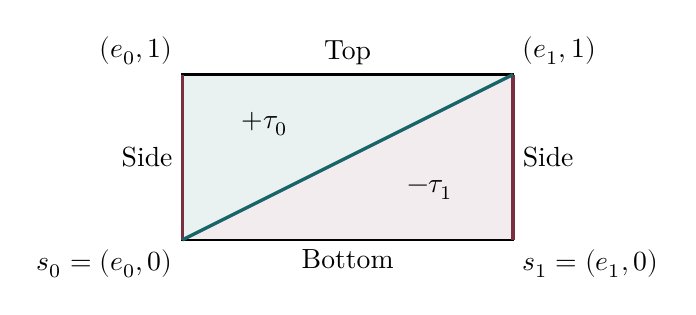
\begin{tikzpicture}[scale=1.05]
\fill[teal!9] (0,0)--(0,2)--(4,2)--cycle;
\fill[burgundy!9] (0,0)--(4,0)--(4,2)--cycle;
\draw[thick] (0,0)--(4,0)--(4,2)--(0,2)--cycle;
\draw[very thick,burgundy] (0,0)--(0,2) (4,0)--(4,2);
\draw[very thick,teal] (0,0)--(4,2);
\node[below left] at (0,0) {$s_0=(e_0,0)$};
\node[below right] at (4,0) {$s_1=(e_1,0)$};
\node[above left] at (0,2) {$(e_0,1)$};
\node[above right] at (4,2) {$(e_1,1)$};
\node at (1,1.4) {$+\tau_0$};\node at (3,.6) {$-\tau_1$};
\node[above] at (2,2) {Top};\node[below] at (2,0) {Bottom};
\node[left] at (0,1) {Side};\node[right] at (4,1) {Side};
\end{tikzpicture}
\]
The open diagonal is inside the square. The vertical edges lie over the boundary points of the base interval. This distinction persists in every dimension.
\end{entry}

\begin{entry}{Definition}{def:prism-operator}{The Prism Operator}
For a singular simplex $\sigma$, define $\sigma_j$ by the composite
\begin{equation*}\label{diag:prism-composite}
\begin{tikzcd}[column sep=small]
\lvert\Delta^{n+1}\rvert\arrow[r,"\tau_j"]&\lvert\Delta^n\rvert\times I
\arrow[r,"\sigma\times\mathrm{id}_I"]&X\times I\arrow[r,"h"]&Y.
\end{tikzcd}
\end{equation*}
Explicitly, the middle map is
\[
\mapdef{\sigma\times\mathrm{id}_I}{\lvert\Delta^n\rvert\times I}{X\times I}{(x,t)}{(\sigma(x),t)}.
\]
The free abelian universal property extends the following assignment uniquely to a homomorphism:
\[
\mapdef{P_n}{C_n(X)}{C_{n+1}(Y)}{\sigma}{\sum_{j=0}^n(-1)^j\sigma_j}.
\]
\end{entry}

\subsection{All Faces and Their Cancellation}\label{sec:faces}
The terms in the boundary are indexed by a Cartesian product:
\[
(j,k)\in\{0,\ldots,n\}\times\{0,\ldots,n+1\},
\qquad
\partial_{n+1}P_n(\sigma)
=\sum_{j=0}^n\sum_{k=0}^{n+1}(-1)^{j+k}\sigma_jd^k.
\]
The first index chooses the prism piece; the second deletes its vertex in position $k$. Each corresponding affine face has type
\[
\tau_jd^k:\lvert\Delta^n\rvert\longrightarrow\lvert\Delta^n\rvert\times I.
\]
The base vertex $e_j$ appears twice in the piece, in positions $j$ and $j+1$. Every other base vertex appears once. This observation classifies all faces:
\[
\begin{array}{c c l}
\text{Kind}&(j,k)&\text{What Remains}\\\hline
\text{Top}&(0,0)&\text{all vertices at height }1\\
\text{Bottom}&(n,n+1)&\text{all vertices at height }0\\
\text{Interior}&(j,j+1),(j+1,j+1),\ 0\le j<n&\text{one vertex over every base vertex}\\
\text{Side}&k<j\text{ or }k>j+1&\text{one base vertex missing}
\end{array}
\]
In the third row the pairs are grouped by their common face. Each pair in the full Cartesian product occurs exactly once in this table.

\begin{entry}{Remark}{rem:top-bottom}{Top and Bottom}
For $\epsilon\in\{0,1\}$ the endpoint inclusion of the base is
\[
\mapdef{\iota_\epsilon}{\lvert\Delta^n\rvert}{\lvert\Delta^n\rvert\times I}{x}{(x,\epsilon)}.
\]
The equalities of affine maps, including their signs, are
\[
\tau_0d^0=\iota_1:\lvert\Delta^n\rvert\longrightarrow\lvert\Delta^n\rvert\times I,
\qquad (-1)^{0+0}=+1,
\]
\[
\tau_nd^{n+1}=\iota_0:\lvert\Delta^n\rvert\longrightarrow\lvert\Delta^n\rvert\times I,
\qquad (-1)^{n+n+1}=-1.
\]
After composition with the homotopy, these give $f_1\sigma-f_0\sigma$.
\end{entry}

\begin{entry}{Remark}{rem:interior-faces}{Interior Faces}
For $0\le j<n$, the two faces
\[
\tau_jd^{j+1}=\tau_{j+1}d^{j+1}:\lvert\Delta^n\rvert\longrightarrow\lvert\Delta^n\rvert\times I
\]
have the same ordered vertices:
\[
(e_0,0),\ldots,(e_j,0),(e_{j+1},1),\ldots,(e_n,1).
\]
They are equal as parametrized simplices, not merely as subsets. The equality is the commutative square
\begin{equation*}\label{diag:interior}
\begin{tikzcd}
\lvert\Delta^n\rvert\arrow[r,"d^{j+1}"]\arrow[d,"d^{j+1}"']&\lvert\Delta^{n+1}\rvert\arrow[d,"\tau_j"]\\
\lvert\Delta^{n+1}\rvert\arrow[r,"\tau_{j+1}"']&\lvert\Delta^n\rvert\times I.
\end{tikzcd}
\end{equation*}
Why is this an interior face? Its relative interior consists of the combinations with all $n+1$ coefficients positive. There is a vertex over each $e_i$, so every base coordinate $t_i$ is positive. There are vertices at both heights, so
\[
0<t=\sum_{i=j+1}^nt_i<1.
\]
These are precisely the strict inequalities describing the interior of the prism in its affine span. The face separates the two adjacent pieces inside the prism. Its own boundary may still reach the outer boundary, as the endpoints of the diagonal do in the square.

The coefficients of this same ordered face in the two boundaries are
\[
(-1)^j(-1)^{j+1}=-1,\qquad
(-1)^{j+1}(-1)^{j+1}=+1.
\]
Thus the signed prism simplices induce opposite orientations on the face. Their contributions cancel, including after composition with $h$.
\end{entry}

\begin{entry}{Remark}{rem:side-faces}{Side Faces}
Suppose that $i\ne j$. There is only one vertex over $e_i$. Deleting it forces $t_i=0$ everywhere on the face, since all remaining vertices have zero $i$th base coordinate. The face therefore lies in the vertical boundary, over the $i$th face of the base. There are exactly two cases:
\[
\begin{array}{c c c c}
\text{Base Index}&\text{Deleted Vertex}&\text{Position }k&\text{Prism Index on the Base Face}\\\hline
 i<j&(e_i,0)&i&j-1\\
 i>j&(e_i,1)&i+1&j
\end{array}
\]
In the lower-dimensional prism the symbols $\tau_{j-1}$ and $\tau_j$ use the same affine definition, now with source $\lvert\Delta^n\rvert$ and target $\lvert\Delta^{n-1}\rvert\times I$. The two cases give the squares
\begin{equation*}\label{diag:sides}
\begin{tikzcd}[column sep=large]
\lvert\Delta^n\rvert\arrow[r,"d^i"]\arrow[d,"\tau_{j-1}"']&\lvert\Delta^{n+1}\rvert\arrow[d,"\tau_j"]\\
\lvert\Delta^{n-1}\rvert\times I\arrow[r,"d^i\times\mathrm{id}_I"']&\lvert\Delta^n\rvert\times I
\end{tikzcd}
\quad(i<j),
\end{equation*}
\[
\begin{tikzcd}[column sep=large]
\lvert\Delta^n\rvert\arrow[r,"d^{i+1}"]\arrow[d,"\tau_j"']&\lvert\Delta^{n+1}\rvert\arrow[d,"\tau_j"]\\
\lvert\Delta^{n-1}\rvert\times I\arrow[r,"d^i\times\mathrm{id}_I"']&\lvert\Delta^n\rvert\times I
\end{tikzcd}
\quad(i>j).
\]
Both commute because their composites have the same ordered vertices. In the first square, omission of $e_i$ shifts the repeated base vertex down from index $j$ to index $j-1$. In the second, it leaves that index unchanged.

To compare the two sums without introducing another dummy index, now index the terms of $P_{n-1}\partial_n$ by
\[
(i,j)\in\{0,\ldots,n\}\times\{0,\ldots,n-1\}.
\]
Here $i$ selects the base face and $j$ selects its prism piece. The matching term of $\partial_{n+1}P_n$ is specified completely by
\[
\begin{array}{c c c c}
\text{Condition}&\text{Prism Piece and Deleted Position}&\text{Its Sign}&\text{Sign in }P_{n-1}\partial_n\\\hline
 i\le j&(j+1,i)&(-1)^{j+1+i}&(-1)^{i+j}\\
 i>j&(j,i+1)&(-1)^{j+i+1}&(-1)^{i+j}
\end{array}
\]
This is a bijection from the displayed Cartesian product to all side faces. The signs are opposite in both rows. Hence the total side contribution is $-P_{n-1}\partial_n(\sigma)$.
\end{entry}

\begin{result}{Proposition}{prop:boundary-identity}{The Boundary Identity}
For the prism operator of Definition~\ref{def:prism-operator} and every $n\ge0$, with $P_{-1}=0$, one has
\[
\partial_{n+1}P_n+P_{n-1}\partial_n
=f_{1,\#,n}-f_{0,\#,n}:C_n(X)\longrightarrow C_n(Y).
\]
\end{result}
\begin{demonstration}{prop:boundary-identity}
By Remarks~\ref{rem:top-bottom}, \ref{rem:interior-faces}, and \ref{rem:side-faces}, adding the three contributions gives
\[
\partial_{n+1}P_n(\sigma)
=\underbrace{f_1\sigma-f_0\sigma}_{\text{top and bottom}}
\underbrace{-P_{n-1}\partial_n(\sigma)}_{\text{sides}}
+\underbrace{0}_{\text{interior faces}}.
\]
For $n=0$ there is one interval, with its top and bottom endpoints and no other faces. Thus the formula also holds with $P_{-1}=0$. Freeness proves \eqref{eq:prism} in every degree.
\end{demonstration}
By the general homotopy-invariance proposition in Lecture 5, homotopy equivalences induce homology isomorphisms.

\section{First Computations}\label{sec:computations}
\subsection{Components, Points, and Disjoint Unions}
Write $\pi_0^{\mathrm{path}}(X)$ for the set of path components, and $\mathbb Z[E]$ for the free abelian group on a set $E$.
\begin{result}{Proposition}{prop:hzero}{Degree Zero}
There is a natural isomorphism
\[
\mapdef{\eta_X}{H_0(X)}{\mathbb Z[\pi_0^{\mathrm{path}}(X)]}{[x]}{\text{the generator for the component of }x}.
\]
\end{result}
\begin{demonstration}{prop:hzero}
Let $M$ be an abelian group. A homomorphism
\[
\alpha:C_0(X)\longrightarrow M
\]
is an assignment of an element of $M$ to each point. The boundary of a path is its endpoint minus its starting point. Thus $\alpha\partial_1=0$ exactly when the assignment is constant on path components. The cokernel property gives the unique factorization
\[
\begin{tikzcd}
C_1(X)\arrow[r,"\partial_1"]&C_0(X)\arrow[r,"q"]\arrow[dr,"\alpha"']&H_0(X)\arrow[d,"\overline\alpha"]\\&&M.
\end{tikzcd}
\]
This is the free abelian universal property for the set of path components. It proves the isomorphism, and its description on points proves naturality.
\end{demonstration}

\begin{result}{Proposition}{prop:point}{A Point}
For the one-point space $*$,
\[
H_n(*)=\begin{cases}\mathbb Z,&n=0,\\0,&n>0.\end{cases}
\]
\end{result}
\begin{demonstration}{prop:point}
There is exactly one singular simplex in every degree. Hence $C_n(*)=\mathbb Z$, and the differential is
\[
\partial_n:\mathbb Z\longrightarrow\mathbb Z,
\qquad \partial_n(1)=\sum_{i=0}^n(-1)^i
=\begin{cases}1,&n>0\text{ even},\\0,&n\text{ odd}.\end{cases}
\]
The chain complex is
\[
\cdots\longrightarrow\underset{3}{\mathbb Z}
\xrightarrow{0}\underset{2}{\mathbb Z}
\xrightarrow{1}\underset{1}{\mathbb Z}
\xrightarrow{0}\underset{0}{\mathbb Z}\longrightarrow0,
\]
where the labels below the groups are their degrees. Kernels modulo images give the asserted groups.
\end{demonstration}

\begin{result}{Proposition}{prop:union}{Disjoint Unions}
For a family $(X_i)_{i\in J}$, the summand inclusions induce isomorphisms
\[
\bigoplus_{i\in J}C_\bullet(X_i)\xrightarrow{\ \cong\ }
C_\bullet\!\left(\coprod_{i\in J}X_i\right),
\qquad
\bigoplus_{i\in J}H_n(X_i)\xrightarrow{\ \cong\ }
H_n\!\left(\coprod_{i\in J}X_i\right).
\]
\end{result}
\begin{demonstration}{prop:union}
Each singular simplex has connected nonempty domain, so its image lies in one summand of the disjoint union. The generators therefore split by summand, and every face stays in the same summand. This proves the chain isomorphism. In a direct sum every element has finite support, so both cycles and boundaries are direct sums of the cycles and boundaries in the summands. Taking their quotient proves the homology isomorphism.
\end{demonstration}

The same argument splits singular chains over path components, even when those components are not open: a simplex has path connected domain and hence lies in one path component, with its subspace topology. In particular, for a discrete space $E$,
\[
H_0(E)=\mathbb Z[E],\qquad H_n(E)=0\quad(n>0).
\]
For the empty space all chain and homology groups are zero.

\subsection{Contractible Spaces and Deformation Retractions}
A space is \emph{contractible} if it is nonempty and its identity is homotopic to a constant map.
\begin{result}{Proposition}{prop:contractible}{Contractible Spaces}
For a contractible space $X$,
\[
H_0(X)\cong\mathbb Z,\qquad H_n(X)=0\quad(n>0).
\]
\end{result}
\begin{demonstration}{prop:contractible}
Choose a point $x_0$ to which $X$ contracts. The maps
\[
f:X\longrightarrow *,\qquad
\mapdef{g}{*}{X}{*}{x_0}
\]
satisfy $fg=\mathrm{id}_*$ and $gf\simeq\mathrm{id}_X$. Their induced maps
\[
f_*:H_n(X)\longrightarrow H_n(*),\qquad
 g_*:H_n(*)\longrightarrow H_n(X)
\]
are therefore inverse isomorphisms. Apply \hyperref[prop:point]{the computation for a point}.
\end{demonstration}

For a nonempty convex subset $V\subseteq\mathbb R^m$ and $x_0\in V$, the contraction is
\[
\mapdef{h}{V\times I}{V}{(x,t)}{(1-t)x+tx_0}.
\]
This applies to Euclidean spaces, balls, intervals, and standard simplices. It also applies when $V$ is star-shaped about $x_0$, meaning that it contains the line segment joining $x_0$ to each of its points.

A \emph{deformation retraction} consists of maps
\[
i:X'\hookrightarrow X,\qquad r:X\longrightarrow X',\qquad
h:X\times I\longrightarrow X
\]
satisfying
\[
ri=\mathrm{id}_{X'},\qquad h(x,0)=x,\qquad h(x,1)=ir(x),\qquad
h(i(x'),t)=i(x').
\]
Then $i$ and $r$ are homotopy inverse maps, so
\[
i_*:H_n(X')\longrightarrow H_n(X),\qquad
r_*:H_n(X)\longrightarrow H_n(X')
\]
are inverse isomorphisms. For example,
\[
\mapdef{r}{\mathbb R\setminus\{0\}}{\{-1,1\}}{x}{x/|x|},
\]
\[
\mapdef{h}{(\mathbb R\setminus\{0\})\times I}{\mathbb R\setminus\{0\}}
{(x,t)}{(1-t)x+t\,x/|x|}
\]
give a deformation retraction. The interpolation remains in the half-line containing $x$. Thus the homology is $\mathbb Z^2$ in degree zero and zero in positive degrees. Removing $m$ distinct points from $\mathbb R$ similarly leaves $m+1$ contractible components.

\section{Relative Chains and the Interval}\label{sec:relative}
\subsection{Pairs, Quotients, and the Exact Sequence}
A pair is a subspace inclusion
\[
i:X'\hookrightarrow X.
\]
Write $(X,X')$ for this pair. The induced inclusion identifies the singular chains of $X'$ with a subcomplex. Define
\[
C_\bullet(X,X')=C_\bullet(X)/C_\bullet(X'),\qquad
H_n(X,X')=H_n(C_\bullet(X,X')).
\]
A map of pairs is a commutative square
\[
\begin{tikzcd}
X'\arrow[r,hook,"i_X"]\arrow[d,"f'"']&X\arrow[d,"f"]\\
Y'\arrow[r,hook,"i_Y"']&Y.
\end{tikzcd}
\]
The relative chain complex is a cokernel. For any chain complex $B_\bullet$ and chain map
\[
u:C_\bullet(X)\longrightarrow B_\bullet,\qquad u i_\#=0,
\]
there is a unique induced map
\[
\overline u:C_\bullet(X,X')\longrightarrow B_\bullet
\]
making the right square commute; the left square is a pushout:
\[
\begin{tikzcd}
C_\bullet(X')\arrow[r,"i_\#"]\arrow[d]&C_\bullet(X)\arrow[r,"u"]\arrow[d,"q"]&B_\bullet\arrow[d,equal]\\
0\arrow[r]&C_\bullet(X,X')\arrow[r,"\overline u"']&B_\bullet.
\end{tikzcd}
\]
For a map of pairs this constructs the relative chain map in the square
\[
\begin{tikzcd}
C_\bullet(X)\arrow[r,"q_X"]\arrow[d,"f_\#"']&C_\bullet(X,X')\arrow[d,"f_\#"]\\
C_\bullet(Y)\arrow[r,"q_Y"']&C_\bullet(Y,Y').
\end{tikzcd}
\]
Uniqueness gives compatibility with identities and composition, hence functoriality.

A relative cycle is represented by $c\in C_n(X)$ with $\partial_nc\in C_{n-1}(X')$. Two such representatives have the same relative homology class exactly when their difference is a boundary in $X$ plus a chain in $X'$.

\begin{result}{Theorem}{thm:relative}{The Long Exact Sequence}
Every pair has a natural exact sequence
\[
\cdots\longrightarrow H_n(X')\xrightarrow{i_*}H_n(X)
\xrightarrow{q_*}H_n(X,X')\xrightarrow{\delta_n}H_{n-1}(X')\longrightarrow\cdots
\]
ending in
\[
H_0(X')\xrightarrow{i_*}H_0(X)\xrightarrow{q_*}H_0(X,X')\longrightarrow0.
\]
The connecting homomorphism is
\[
\mapdef{\delta_n}{H_n(X,X')}{H_{n-1}(X')}{[c]}{[\partial_nc]}.
\]
\end{result}
\begin{demonstration}{thm:relative}
Apply the long exact sequence of chain complexes from Lecture 2 to
\[
0\longrightarrow C_\bullet(X')\xrightarrow{i_\#}C_\bullet(X)
\xrightarrow{q}C_\bullet(X,X')\longrightarrow0.
\]
For a relative cycle, $\partial_nc$ lies in the subcomplex and is a cycle because $\partial_{n-1}\partial_n=0$. Replacing $c$ by $c+\partial_{n+1}b+c'$ with $c'\in C_n(X')$ changes its boundary by $\partial_nc'$, so the connecting class is well defined. The chain-complex theorem supplies exactness and naturality.
\end{demonstration}

\begin{entry}{Example}{ex:interval-endpoints}{The Interval and Its Endpoints}
Take $X=I$ and $X'=\partial I=\{0,1\}$. Contractibility of $I$ and the computation for discrete spaces reduce the exact sequence to
\[
0\longrightarrow H_1(I,\partial I)\xrightarrow{\delta_1}\mathbb Z^2
\xrightarrow{\varepsilon}\mathbb Z\longrightarrow H_0(I,\partial I)\longrightarrow0,
\]
where
\[
\mapdef{\varepsilon}{\mathbb Z^2}{\mathbb Z}{(a,b)}{a+b}.
\]
Both endpoint generators map to the component generator of $I$. The map is surjective, and its kernel is $\mathbb Z(-1,1)$. Thus
\[
H_n(I,\partial I)=\begin{cases}\mathbb Z,&n=1,\\0,&n\ne1.\end{cases}
\]
The singular edge
\[
\mapdef{e}{|\Delta^1|}{I}{(t_0,t_1)}{t_1}
\]
has boundary equal to the point generator at $1$ minus the point generator at $0$. Thus $\delta_1[e]=(-1,1)$ and $[e]$ is a generator.

Reflection is the map of pairs induced by
\[
\mapdef{\rho}{I}{I}{t}{1-t},\qquad
\mapdef{\rho'}{\partial I}{\partial I}{t}{1-t}.
\]
Naturality gives
\[
\begin{tikzcd}
H_1(I,\partial I)\arrow[r,"\delta_1"]\arrow[d,"\rho_*"']&H_0(\partial I)\arrow[d,"\rho'_*"]\\
H_1(I,\partial I)\arrow[r,"\delta_1"']&H_0(\partial I).
\end{tikzcd}
\]
The right map exchanges the endpoint generators, sending $(-1,1)$ to its negative. Injectivity of $\delta_1$ therefore gives $\rho_*[e]=-[e]$.
\end{entry}

\subsection{Relative Homotopies and Reduced Homology}
\begin{result}{Proposition}{prop:relative-invariance}{Homotopies of Pairs}
Suppose that
\[
f_0,f_1:(X,X')\longrightarrow(Y,Y')
\]
are joined by a homotopy
\[
h:X\times I\longrightarrow Y,\qquad h(X'\times I)\subseteq Y'.
\]
Then the induced maps agree:
\[
f_{0,*}=f_{1,*}:H_n(X,X')\longrightarrow H_n(Y,Y').
\]
\end{result}
\begin{demonstration}{prop:relative-invariance}
For a simplex in $X'$, all its prism simplices have image in $Y'$. Hence the prism homomorphisms restrict and descend:
\[
P_n:C_n(X')\longrightarrow C_{n+1}(Y'),\qquad
\overline P_n:C_n(X,X')\longrightarrow C_{n+1}(Y,Y').
\]
Identity \eqref{eq:prism} descends to the quotient. It makes the relative chain maps chain homotopic, so they induce equal homology maps.
\end{demonstration}

The subspace condition is essential. The contraction
\[
\mapdef{h}{I\times I}{I}{(x,t)}{(1-t)x}
\]
moves the endpoint $1$ into the interior for $0<t<1$. It is therefore not a homotopy of the pair $(I,\partial I)$.

For a nonempty space $X$, the augmentation is the chain map
\[
\varepsilon:C_\bullet(X)\longrightarrow\mathbb Z[0],
\]
whose degree-zero component is
\[
\mapdef{\varepsilon_0}{C_0(X)}{\mathbb Z}{\sum_i a_i x_i}{\sum_i a_i},
\]
and whose positive-degree components are zero. Here $\mathbb Z[0]$ is concentrated in degree zero. Every path boundary has coefficient sum zero, so this is a chain map. It is surjective because $X$ is nonempty.

Define reduced chains by the kernel, equivalently by the pullback:
\[
\begin{tikzcd}
\widetilde C_\bullet(X)\arrow[r]\arrow[d]&C_\bullet(X)\arrow[d,"\varepsilon"]\\
0\arrow[r]&\mathbb Z[0].
\end{tikzcd}
\]
Their homology is $\widetilde H_n(X)$. The kernel exact sequence gives
\[
\widetilde H_n(X)\cong H_n(X)\quad(n>0),\qquad
\widetilde H_0(X)=\ker\bigl(\varepsilon_*:H_0(X)\longrightarrow\mathbb Z\bigr).
\]
The prism homomorphisms restrict to the reduced complexes, so reduced homology is homotopy invariant.

If $X$ is contractible and $X'$ is nonempty, the exact sequence of the pair gives isomorphisms
\[
\delta_n:H_n(X,X')\xrightarrow{\ \cong\ }\widetilde H_{n-1}(X')\quad(n\ge1),
\qquad H_0(X,X')=0.
\]
For $n\ge2$ both adjacent positive-degree groups of $X$ vanish. For $n=1$ the image of $\delta_1$ is the kernel of the augmentation on $H_0(X')$.

For example, let $X'$ be a finite discrete subspace consisting of $m\ge1$ points in a contractible space $X$. Then
\[
H_1(X,X')\cong\ker\bigl(\varepsilon:\mathbb Z^m\longrightarrow\mathbb Z\bigr)
\cong\mathbb Z^{m-1},
\]
where $\varepsilon$ sums the coordinates; all other relative groups vanish. Choose one marked point and paths from it to the others. Their relative classes form a basis because their boundaries are a basis of the augmentation kernel. In particular, three marked points in an interval or a disk give relative first homology $\mathbb Z^2$.

The next lecture will compute the homology of circles and spheres using open covers. The geometric input will be subdivision: chains whose simplices lie in individual members of an open cover compute the same homology as all singular chains. The long exact sequence will then turn this fact into the Mayer--Vietoris sequence.
\end{document}
